\documentclass[11pt, a4paper, landscape]{article}

% essential packages
\usepackage[T1]{fontenc}
\usepackage{lmodern}
\usepackage[UKenglish]{babel}
\usepackage{csquotes}
\usepackage{graphicx}
\usepackage{hyperref}
\usepackage{amsmath}
\usepackage{amssymb}
\usepackage{booktabs}
\usepackage{longtable}
\usepackage{xcolor}
\usepackage{listings}
\usepackage{enumitem}

% additional packages for layout and formatting
\usepackage[landscape, margin=12mm]{geometry}
\usepackage{tcolorbox}
\usepackage{multicol}
\usepackage{tikz}
\usepackage{array}
\usepackage{tabularx}
\usepackage{fancyhdr}

% define colors from the html
\definecolor{mainblue}{HTML}{0066CC}
\definecolor{optiongreen}{HTML}{006600}
\definecolor{lightblue}{HTML}{E8F4F8}
\definecolor{lightgray}{HTML}{F5F5F5}
\definecolor{darkgray}{HTML}{666666}
\definecolor{bordercolor}{HTML}{DDDDDD}

% spacing
\frenchspacing
\setlength{\parindent}{0pt}
\setlength{\parskip}{2.5mm}

% remove page numbering
\pagenumbering{gobble}

% custom commands for formatting
\newcommand{\slcmd}[1]{\textcolor{mainblue}{\texttt{\textbf{#1}}}}
\newcommand{\slopt}[1]{\textcolor{optiongreen}{\texttt{#1}}}

% reduce vertical spacing slightly
\renewcommand{\baselinestretch}{0.95}

% title and metadata
\title{Slurm Job Scheduler Reference Card}
\date{}

\begin{document}

% page 1
\begin{center}
\Large\textbf{Slurm Job Scheduler Reference Card}
\end{center}
\vspace{-2mm}
\noindent\rule{\linewidth}{3pt}

\vspace{4mm}

% reminder box
\begin{tcolorbox}[colback=lightblue, colframe=mainblue, boxrule=2pt, arc=5mm, left=5mm, right=5mm, top=3mm, bottom=3mm]
\centering
\normalsize\textbf{These commands only work on the HPC system - first connect with: ssh wilson}
\end{tcolorbox}

\vspace{3mm}

% essential slurm commands section
\begin{tcolorbox}[colback=white, colframe=bordercolor, boxrule=1pt, arc=5mm, left=4mm, right=4mm, top=4mm, bottom=4mm]
\textbf{\large Essential Slurm Commands}\\[-3mm]
\textcolor{mainblue}{\rule{\dimexpr\linewidth-8mm\relax}{2pt}}
\vspace{2mm}

\small
\begin{tabular}{@{}p{0.48\textwidth}p{0.48\textwidth}@{}}
\slcmd{sbatch} \slopt{submit\_job.sh} & Submit a job script to the queue \\[1.5mm]
\slcmd{squeue} & Display all jobs in the queue \\[1.5mm]
\slcmd{squeue} \slopt{-{}-me} & Display only your jobs \\[1.5mm]
\slcmd{squeue} \slopt{-u <FEDID>} & Display jobs for a specific user \\[1.5mm]
\slcmd{scancel} \slopt{<JOBID>} & Cancel a specific job \\[1.5mm]
\slcmd{scancel} \slopt{-{}-me} & Cancel all your jobs \\[1.5mm]
\slcmd{sacct} \slopt{-j <JOBID>} & View accounting information for a job \\[1.5mm]
\end{tabular}
\end{tcolorbox}

\vspace{2.5mm}

% understanding queue status section
\begin{tcolorbox}[colback=white, colframe=bordercolor, boxrule=1pt, arc=5mm, left=4mm, right=4mm, top=4mm, bottom=4mm]
\textbf{\large Understanding Queue Status (squeue output)}\\[-3mm]
\textcolor{mainblue}{\rule{\dimexpr\linewidth-8mm\relax}{2pt}}
\vspace{2mm}

% output box
\begin{tcolorbox}[colback=lightgray, colframe=bordercolor, boxrule=1pt, arc=3mm, left=3mm, right=3mm, top=3mm, bottom=3mm]
\small\ttfamily
JOBID~~PARTITION~~NAME~~~~~USER~~~ST~~TIME~~~~~NODES\\
12345~~cs05r~~~~~~gpu\_job~~user1~~R~~~0:07:21~~1\\
12346~~cs05r~~~~~~test~~~~~user2~~PD~~0:00:00~~1
\end{tcolorbox}

\vspace{2.5mm}

\small
\begin{tabular}{@{}p{0.25\textwidth}p{0.71\textwidth}@{}}
\textbf{JOBID} & Unique job identifier (use this for scancel/sacct) \\[1mm]
\textbf{ST (Status)} & \textbf{R} = Running, \textbf{PD} = Pending, \textbf{CG} = Completing, \textbf{CD} = Completed \\[1mm]
\textbf{TIME} & How long the job has been running (HH:MM:SS) \\[1mm]
\textbf{NODES} & Number of compute nodes allocated to the job \\
\end{tabular}
\end{tcolorbox}

\vfill
\newpage

% page 2
% sample gpu job submission script
\begin{tcolorbox}[colback=white, colframe=bordercolor, boxrule=1pt, arc=5mm, left=4mm, right=4mm, top=4mm, bottom=4mm]
\textbf{\large Sample GPU Job Submission Script}\\[-3mm]
\textcolor{mainblue}{\rule{\dimexpr\linewidth-8mm\relax}{2pt}}
\vspace{2mm}

% script box
\begin{tcolorbox}[colback=lightgray!50, colframe=bordercolor!70, boxrule=2pt, arc=4mm, left=3mm, right=3mm, top=2mm, bottom=2mm]
\small\ttfamily
\begin{tabbing}
\#!/usr/bin/env bash\\
\#SBATCH -{}-job-name=my\_gpu\_job \hspace{8mm} \= \# name for your job\\
\#SBATCH -{}-partition=cs05r \> \# GPU partition\\
\#SBATCH -{}-time=00:10:00 \> \# time limit (HH:MM:SS)\\
\#SBATCH -{}-gpus-per-node=1 \> \# request 1 GPU\\
\#SBATCH -{}-mem=8G \> \# memory required\\
\\
\# load any required modules here\\
module load python/3.9\\
\\
\# run your Python script\\
python my\_gpu\_script.py
\end{tabbing}
\end{tcolorbox}
\end{tcolorbox}

\vspace{3mm}

% monitoring job output section
\begin{tcolorbox}[colback=white, colframe=bordercolor, boxrule=1pt, arc=5mm, left=4mm, right=4mm, top=4mm, bottom=4mm]
\textbf{\large Monitoring Job Output}\\[-3mm]
\textcolor{mainblue}{\rule{\dimexpr\linewidth-8mm\relax}{2pt}}
\vspace{2mm}

\small
\begin{tabular}{@{}p{0.48\textwidth}p{0.48\textwidth}@{}}
\slcmd{cat} \slopt{slurm-12345.out} & View the entire output file \\[1.5mm]
\slcmd{tail} \slopt{slurm-12345.out} & View the last 10 lines of output \\[1.5mm]
\slcmd{tail -f} \slopt{slurm-12345.out} & Watch output in real-time (Ctrl+C to exit) \\[1.5mm]
\slcmd{head} \slopt{slurm-12345.out} & View the first 10 lines of output \\
\end{tabular}
\end{tcolorbox}

\vspace{3mm}

% typical hpc workflow section
\begin{tcolorbox}[colback=white, colframe=bordercolor, boxrule=1pt, arc=5mm, left=4mm, right=4mm, top=4mm, bottom=4mm]
\textbf{\large Typical HPC Workflow}\\[-3mm]
\textcolor{mainblue}{\rule{\dimexpr\linewidth-8mm\relax}{2pt}}
\vspace{3mm}

% workflow boxes
\begin{center}
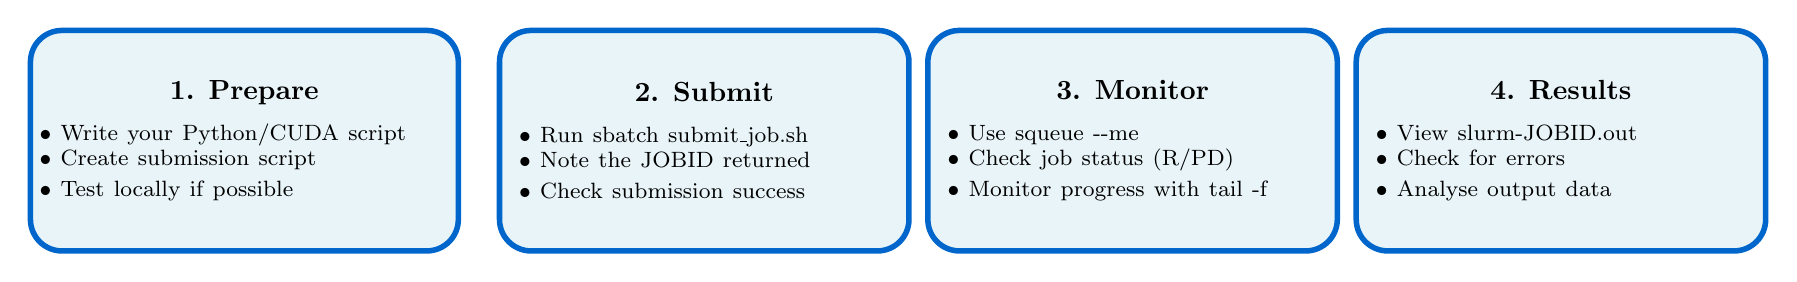
\begin{tikzpicture}[scale=0.8]
% step 1
\node[draw=mainblue, fill=lightblue, rounded corners=4mm, minimum width=5.2cm, minimum height=2.8cm, text width=5.2cm, align=left, line width=2pt] (step1) at (0,0) {
\centering\textbf{\normalsize 1. Prepare}\\[2mm]
\raggedright
\footnotesize
$\bullet$ Write your Python/CUDA script\\
$\bullet$ Create submission script\\
$\bullet$ Test locally if possible
};

% arrow 1
%\node[mainblue] at (3.4,0) {\Large$\rightarrow$};

% step 2
\node[draw=mainblue, fill=lightblue, rounded corners=4mm, minimum width=5.2cm, minimum height=2.8cm, text width=4.7cm, align=left, line width=2pt] (step2) at (7.3,0) {
\centering\textbf{\normalsize 2. Submit}\\[2mm]
\raggedright
\footnotesize
$\bullet$ Run sbatch submit\_job.sh\\
$\bullet$ Note the JOBID returned\\
$\bullet$ Check submission success
};

% arrow 2
%\node[mainblue] at (10.2,0) {\Large$\rightarrow$};

% step 3
\node[draw=mainblue, fill=lightblue, rounded corners=4mm, minimum width=5.2cm, minimum height=2.8cm, text width=4.7cm, align=left, line width=2pt] (step3) at (14.1,0) {
\centering\textbf{\normalsize 3. Monitor}\\[2mm]
\raggedright
\footnotesize
$\bullet$ Use squeue -{}-me\\
$\bullet$ Check job status (R/PD)\\
$\bullet$ Monitor progress with tail -f
};

% arrow 3
%\node[mainblue] at (17,0) {\Large$\rightarrow$};

% step 4
\node[draw=mainblue, fill=lightblue, rounded corners=4mm, minimum width=5.2cm, minimum height=2.8cm, text width=4.7cm, align=left, line width=2pt] (step4) at (20.9,0) {
\centering\textbf{\normalsize 4. Results}\\[2mm]
\raggedright
\footnotesize
$\bullet$ View slurm-JOBID.out\\
$\bullet$ Check for errors\\
$\bullet$ Analyse output data
};
\end{tikzpicture}
\end{center}
\end{tcolorbox}

\vspace{3mm}

%% tips section - two columns
%\begin{multicols}{2}
%\begin{tcolorbox}[colback=white!95, colframe=bordercolor, boxrule=1pt, arc=4mm, left=4mm, right=4mm, top=4mm, bottom=4mm]
%\textbf{\normalsize Common Issues}\\[2mm]
%\footnotesize
%$\bullet$ Job stays in PD (Pending)? Check partition availability with \slcmd{sinfo}\\
%$\bullet$ Script not found? Check file permissions: \slcmd{chmod +x submit\_job.sh}\\
%$\bullet$ Out of memory? Increase \slopt{-{}-mem} in your script
%\end{tcolorbox}

%\begin{tcolorbox}[colback=white!95, colframe=bordercolor, boxrule=1pt, arc=4mm, left=4mm, right=4mm, top=4mm, bottom=4mm]
%\textbf{\normalsize Best Practices}\\[2mm]
%\footnotesize
%$\bullet$ Always specify a time limit to avoid blocking resources\\
%$\bullet$ Use meaningful job names to identify your jobs easily\\
%$\bullet$ Check your output files for errors before assuming success
%\end{tcolorbox}
%\end{multicols}

\end{document}
